\newcommand{\texCommand}[1]{\texttt{\textbackslash{#1}}}%

\newcommand{\exemplo}[1]{%
\vspace{\baselineskip}%
\noindent\fbox{\begin{minipage}{\textwidth}#1\end{minipage}}%
\\\vspace{\baselineskip}}%

\newcommand{\exemploVerbatim}[1]{%
\vspace{\baselineskip}%
\noindent\fbox{\begin{minipage}{\textwidth}%
#1\end{minipage}}%
\\\vspace{\baselineskip}}%


Este capítulo descreve a classe \unbcic, e demonstra os comandos disponíveis. A
última versão foi atualizada pelo Prof. Ralha, em 2008 (vide \refAnexo{Anexo1}).
A melhor forma de entender o funcionamento é observar o arquivo principal deste
documento (\texttt{monografia.tex}).

%%%%%%%%%%%%%%%%%%%%%%%%%%%%%%%%%%%%%%%%%%%%%%%%%%%%%%%%%%%%%%%%%%%%%%%%%%%%%%%%
%%%%%%%%%%%%%%%%%%%%%%%%%%%%%%%%%%%%%%%%%%%%%%%%%%%%%%%%%%%%%%%%%%%%%%%%%%%%%%%%
%%%%%%%%%%%%%%%%%%%%%%%%%%%%%%%%%%%%%%%%%%%%%%%%%%%%%%%%%%%%%%%%%%%%%%%%%%%%%%%%
\section{Biometria} \label{sec:fundamentacao:biometria}

\par Biometria são medidas físicas ou comportamentais que identificam um indivíduo unicamente \cite{li2009encyclopedia}. Nas últimas décadas, com os avanços das tecnologias, foi possível implementar sistemas de autenticação biométrica para identificar pessoas \cite{wayman2005biometric}. 

\par As Subseções \ref{sec:fundamentacao:biometria:caracteristicas} e \ref{sec:fundamentacao:biometria:criterios} explicam com mais detalhes quais as características biométricas existem e os critérios utilizados para determinar quais são as melhores, respectivamente. Sistemas biométricos são melhores explicados na Seção \ref{sec:fundamentacao:sis_bio}.

\subsection{Características biométricas}\label{sec:fundamentacao:biometria:caracteristicas}

\par Características biométricas são as medidas que identificam unicamente uma pessoa. Podem ser divididas em três categorias: físicas, comportamentais e híbridas \cite{li2009encyclopedia}.

\par Características físicas são aspectos fisiológicos do corpo humano. Como medidas, padrões, cores ou
formatos. Algumas das características físicas mais utilizadas são:

\begin{itemize}
    \item Impressão digital;
    \item Íris;
    \item Rosto;
    \item Formato das mãos;
    \item Veias das maos;
    \item Formato da orelha;
    \item Retina.
\end{itemize}

\par Características comportamentais, são aspectos psicológicos. Como fatores que levam pessoas a praticarem atividades ou ações que as distinguem unicamente \cite{wayman2005biometric}. Alguns dos aspectos comportamentais utilizados para autenticação biométrica são:

\begin{itemize}
    \item Assinatura;
    \item Forma de caminhar.
\end{itemize}

\par Já características híbridas, são aspectos que envolvem tanto fatores fisiológicos quanto comportamentais. A característica híbrida mais utilizada em aplicações na atualidade é a voz. Tamanho e formato da boca, garganta, cavidade nasal e outros fatores físicos influenciam diretamente na frequência da voz da pessoa, mas, fatores comportamentais como humor, idioma e sotaque também são essencias para a diferenciação da voz de indivíduos.

\subsection{Qualidade das características biométricas} \label{sec:fundamentacao:biometria:criterios}

\par Como explicado na Seção \ref{sec:fundamentacao:biometria:caracteristicas}, existem inúmeras características biométricas. Não há consenso para qual a melhor, mas cada uma possui vantagens e desvantagens para a utilização em autenticação biométrica. Cinco critérios são utilizados para avaliar a qualidade das características biométricas \cite{wayman2001}:

\begin{enumerate}
    \item Aceitabilidade: Característica que não sofreria objeções das pessoas para adquirí-la;
    \item Robustez: Característica que não sofre mudanças ao longo do tempo, ou seja, imutável;
    \item Disponibilidade: Característica que todo ser humano deveria possuir;
    \item Distintividade: Característica que possui grande variação em uma população;
    \item Acessibilidade: Característica que pode ser facilmente adquirida por meio de sensores.
\end{enumerate}

\par A \refTab{tab:fundamentacao:biometria:criterio} ilustra a comparação das características listadas na Seção \ref{sec:fundamentacao:biometria:caracteristicas} com os cinco critérios enumerados acima \cite{mali2013}.

\tabela{Comparação das características biométricas}{tab:fundamentacao:biometria:criterio}{|l|l|l|l|l|l|}{
\hline
\textbf{Biometria} & \textbf{1 - Aceit.} & \textbf{2 - Rob.} & \textbf{3 - Dispon.} & \textbf{4 - Distint.} & \textbf{5 - Acess.} \\ \hline
Impressão digital & Médio & Alto & Médio & Alto & Médio \\ \hline
Íris & Baixo & Alto & Alto & Alto & Médio \\ \hline
Rosto & Alto & Médio & Alto & Baixo & Alto \\ \hline
Formato das mãos & Médio & Médio & Médio & Médio & Alto \\ \hline
Veias das Médioãos & Médio & Médio & Médio & Médio & Médio \\ \hline
Formato da orelha & Alto & Alto & Alto & Médio & Médio \\ \hline
Retina & Baixo & Médio & Alto & Alto & Baixo \\ \hline
Assinatura & Alto & Baixo & Baixo & Baixo & Alto \\ \hline
Forma de caminhar & Alto & Baixo & Médio & Baixo & Alto \\ \hline
Voz & Alto & Baixo & Médio & Baixo & Médio \\ \hline
}

\section{Sistemas biométricos}\label{sec:fundamentacao:sis_bio}

\par Sistemas biométricos são sistemas tecnológicas usados para identificar pessoas por meio de autenticação biométrica e são projetados para duas hipóteses \cite{wayman2005biometric}: 

\begin{enumerate}
    \item Positivas: Amostras submetidas ao sistema pertencem a uma pessoa registrada;
    \item Negativas: Amostras submetidas ao sistema pertencem a uma pessoa não registrada.
\end{enumerate}

\par Podem ser usadas inúmeras características biométricas, como as listadas na Seção \ref{sec:fundamentacao:biometria:caracteristicas}. Ter inúmeros objetivos, como procurar por pessoas conhecidas ou desconhecidas e verificar se a pessoa é ou não é quem afirma que é. Podem ser utilizados, também, em diferentes ambientes, como ao ar livre ou dentro de algum local, ambientes controlados ou não e com o manuseio ou não de pessoas treinadas para usar o sistema \cite{wayman2005biometric}. As aplicações são as mais variadas, mas são utilizados principalmente para controle de acesso de pessoas em locais ou aplicações.

\par Sistemas biométricos tipicamente consistem em dois métodos \cite{wayman2005biometric}:

\begin{itemize}
    \item Verificação (\textit{Intraclasse}): Usuário informa quem é, insere sua característica biométrica e então comparações são feitas apenas entre as características registradas do usuário com a inserida, verificando se há ou não correspondência;
    \item Identificação (\textit{Interclasse}): Usuário insere sua característica biométrica e é comparada com todas as registradas no sistema, verificando se há ou não correspondência.
\end{itemize}

\par Os métodos não precisam ser usados individualmente, podendo haver sistemas híbridos, mas em sistemas negativos, apenas o método de identificação é possível \cite{wayman2005biometric}.

\par A \refFig{fig:sis_bio:arquitetura} ilustra a arquitetura de um sistema biométrico generalizado. O uso de sistemas biométricos consiste em duas etapas: registro e autenticação. O registro é a etapa em que a característica biométrica da pessoa que está usando pela primeira vez o sistema é processada e registrada. Já a autenticação, é a etapa em que uma pessoa cadastrada disponibiliza a característica biométrica para o sistema de forma a verificar se é ou não registrada.

\par Cada um dos blocos do diagrama apresentado na \refFig{fig:sis_bio:arquitetura} são explicados nas Seções \ref{sec:sis_bio:coleta} até \ref{sec:sis_bio:decisao}.

\figura[h!]{img/arquitetura_biometria}{Arquitetura de um sistema biométrico genérico}{fig:sis_bio:arquitetura}{width=1\textwidth}

\subsection{Coleta} \label{sec:sis_bio:coleta}

\par Módulo de sistemas biométricos responsável por capturar sinais de uma característica biométrica por meio de um sensor eletrônico \cite{wayman2005biometric}. O resultado apresentado pelo sensor, que vai ser posteriormente processado, é a combinação de três fatores: a medida biométrica, a maneira com que a medida é apresentada (imagem, áudio, vídeo) e os parâmetros técnicos do sensor. Se qualquer um dos três fatores sofre modificação, o desempenho do sistema é impactado.

\par A \refFig{fig:sis_bio:coleta} ilustra alguns modelos de sensores eletônicos utilizados para capturar impressões digitais e formato das mãos, respectivamente.

\figurasDuplas{h!}{img/fingerprint_sensor}{img/hand_sensor}{Sensores biométricos de impressão digital e formato das mãos}{Sensor \textit{Futronic FS80H} (Fonte: \cite{fingerprint_sensor})}{Sensor \textit{Schlage HandPunch HP2000E} (Fonte: \cite{hand_sensor})}{fig:sis_bio:coleta}{fig:sis_bio:coleta:fingerprint}{{fig:sis_bio:coleta:hand}{.5\textwidth}{width=.5\textwidth}}

\subsection{Transmissão}\label{sec:sis_bio:transmissao}

\par Módulo de sistemas biométricos que transmite a característica biométrica capturada pelo sensor no módulo de \textit{Coleta} para ser processada e armazenada \cite{wayman2005biometric}. Esse módulo não precisa estar presente em todo sistema biométrico, apenas os que processam e armazenam os modelos gerados no módulo de \textit{processamento} remotamente.

\par O tamanho dos dados da característica biométrica capturada podem variar, mas geralmente são grandes, e podem causar gargalos na transmissão e ocupar muito espaço de armazenamento. Portanto, técnicas de compressão de dados podem ser aplicadas, para acelerar a transmissão e reduzir o espaço de armazenamento no banco de dados. A compressão, no entanto, introduz desafios, porque causam perda da qualidade dos dados e podem influenciar diretamente nos resultados do módulo de \textit{Processamento} e, consequentemente, no de \textit{decisão}. De forma a reduzir o impacto da compressão, técnicas específicas são aplicadas para cada tipo de característica biométrica.

\par A \refFig{fig:sis_bio:iris_comprimida} ilustra as imagens de uma íris e o resultado da sua compressão usando a técnica \textit{JPEG2000}.

% imagem

\subsection{Processamento}

\par O módulo de processamento consiste em segmentar, extrair os atributos e gerar o modelo da característica biométrica capturada no módulo de coleta \cite{wayman2005biometric}.

\par A segmentação é a etapa responsável por encontrar e separar a característica biométrica no sinal de entrada capturado pelo sensor \cite{wayman2005biometric}. A \refFig{fig:sis_bio:processamento:segmentacao} ilustra os resultados da etapa de segmentação de impressão digital e de uma íris, respectivamente.

% imagens

\par A extração de atributos é a etapa que recebe a característica biométrica segmentada, ignora os ruídos causados pelo sensor, transmissão ou a própria segmentação e a reduz a uma representação matemática com base em seus padrões, comumente chamados de modelos ou \textit{templates} \cite{wayman2005biometric}.

\par Na etapa de registro do sistema, esses \textit{templates} são salvos e associados à pessoa sendo cadastrada em algum banco de dados. Na etapa de autenticação, os \textit{templates} salvos são comparados com o \textit{template} sendo autenticado no módulo de \textit{decisão}.

\subsection{Armazenamento}

\par O módulo de armazenamento é o responsável por armazenar os \textit{templates} das características biométricas geradas no registro de uma pessoa no sistema. Pode ou não, ser um banco de dados centralizado, dependendo da aplicação \cite{wayman2005biometric}.

\par Em sistemas que utilizam a funcionalidade de identificação, é mais comum a utilização de bancos de dados centralizados, enquanto em sistemas de verificação, é mais comum o uso de cartões para armazenar o \textit{template}.

\subsection{Decisão} \label{sec:sis_bio:decisao}

\par O módulo de decisão consiste na comparação dos \textit{templates} de características biométricas armazenadas com o \textit{template} gerado na etapa de autenticação e na decisão se há ou não correspondência para aceitar ou rejeitar a pessoa sendo autenticada no sistema \cite{wayman2005biometric}.

\par A comparação pode ser feita usando métricas de diferença ou similaridade dos \textit{templates}, e varia para cada sistema. Considerando uma distância ou similaridade, a decisão é feita por meio de um limiar. O valor do limiar a ser utilizado no sistema depende da aplicação. Há aplicações de risco e que não podem permitir impostores, de forma que o limiar deve ser mais criterioso. Enquanto há aplicações que não é desejado que pessoas cadastradas sejam negadas frequentemente, e portanto, o limiar deve ser menos criterioso.

%%%%%%%%%%%%%%%%%%%%%%%%%%%%%%%%%%%%%%%%%%%%%%%%%%%%%%%%%%%%%%%%%%%%%%%%%%%%%%%%
%%%%%%%%%%%%%%%%%%%%%%%%%%%%%%%%%%%%%%%%%%%%%%%%%%%%%%%%%%%%%%%%%%%%%%%%%%%%%%%%
%%%%%%%%%%%%%%%%%%%%%%%%%%%%%%%%%%%%%%%%%%%%%%%%%%%%%%%%%%%%%%%%%%%%%%%%%%%%%%%%
\section{Reconhecimento de Íris}

\par Colocar os passos utilziados pelo Daugman \cite{daugman2004}

\par segmentacao

\par Extraçao features

\par Codificação

\par Matching

\subsection{Olho humano}\label{sec:iris:olho}

\par Íris é a parte circular colorida e pigmentada do olho humano. Possui músculos que, ao contrair e dilatar a pupila, controlam a quantidade de luz que entra na retina \cite{adlerIris2003}. A \refFig{fig:olhohumano} ilustra a íris, pupila, retina e as outras estruturas do olho humano.

\figuraBib[!h]{olho-humano}{Anatomia de um olho humano}{imgOlhoHumano}{fig:olhohumano}{width=0.4\textwidth}%

\par A íris apresenta alta variedade de padrões e colorações, que podem variar do azul, castanho, verde, avelã até o cinza. A cor da íris é definida geneticamente, enquanto os padrões não \cite{adlerIris2003}. A íris do olho esquerdo de um indivíduo é necessariamente diferente da do olho direito \cite{wayman2005biometric}. Essa diferença é ilustrada nas \refFigs{fig:iris_direita}{fig:iris_esquerda}.

\par Com a probabilidade de 1 em $10^{72}$ de existirem padrões de íris iguais e não modificarem ao longo da vida, é considerada um dos melhores tipos de biometria \cite{iris_UFRJ}.

\figurasDuplas{h!}{img/iris_direita}{img/iris_esquerda}{Diferança das íris do olho humano}{Íris do olho direito}{íris do olho esquerdo}{fig:olhos}{fig:iris_direita}{{fig:iris_esquerda}{.5\textwidth}{width=.5\textwidth}}

% \begin{figure}[h!]
% \centering
% \begin{subfigure}{.5\textwidth}
%   \centering
%   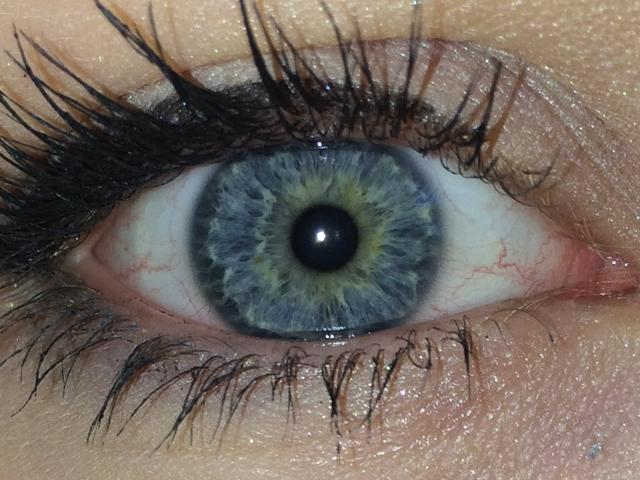
\includegraphics[width=.5\linewidth]{img/iris_direita}
%   \caption{Íris do olho direito.}\label{fig:iris_direita}
% \end{subfigure}%
% \begin{subfigure}{.5\textwidth}
%   \centering
%   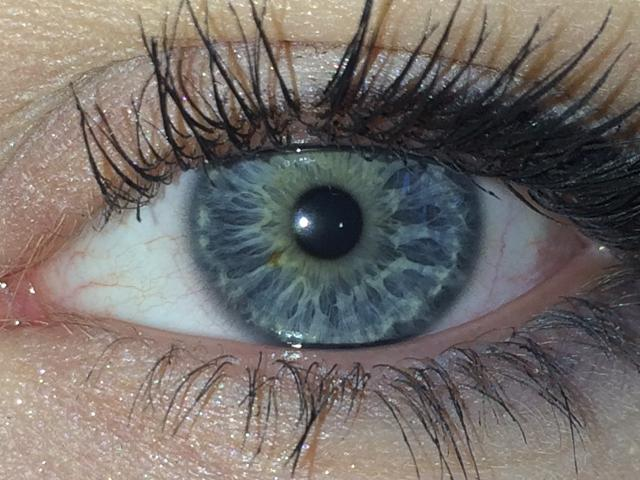
\includegraphics[width=.5\linewidth]{img/iris_esquerda}
%   \caption{Íris do olho esquerdo.}\label{fig:iris_esquerda}
% \end{subfigure}
% \caption{Diferença das íris do olho humano.}
% \label{fig:olhos}
% \end{figure}

% \begin{figure}[!h]
%   \centering
%   \begin{minipage}[b]{0.4\textwidth}
%     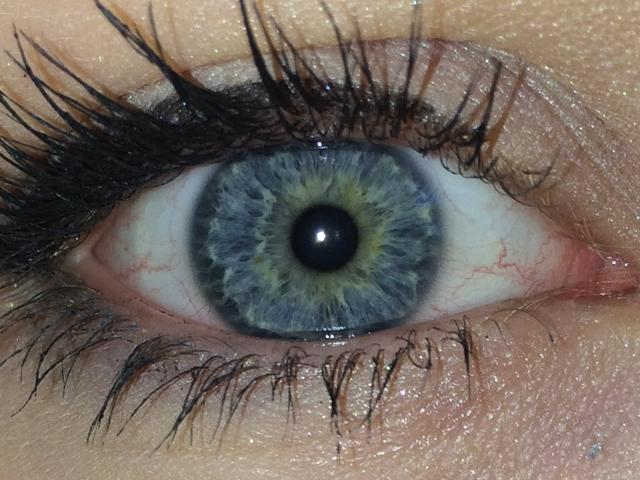
\includegraphics[width=\textwidth]{img/iris_direita.jpg}
%     \caption{Íris do olho direito.}\label{fig:iris_direita}
%   \end{minipage}
%   \hfill
%   \begin{minipage}[b]{0.4\textwidth}
%     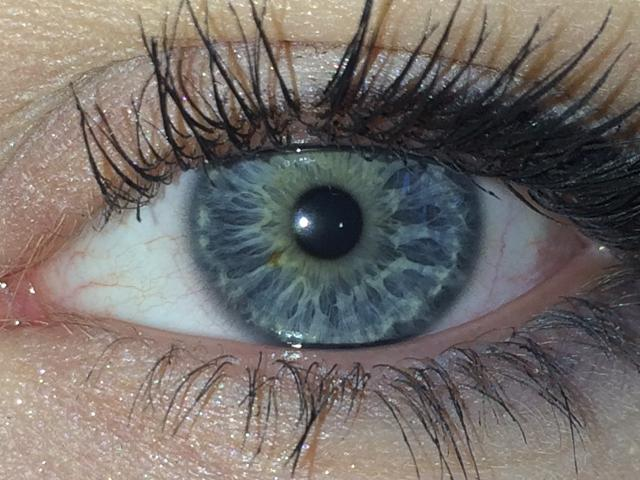
\includegraphics[width=\textwidth]{img/iris_esquerda.jpg}
%     \caption{Íris do olho esquerdo.}\label{fig:iris_esquerda}
%   \end{minipage}
% \end{figure}

\subsection{\textit{Imagens \acrfull{VL} vs \acrfull{NIR}}}

\par Espectro eletromagnético é o intervalo de ondas que são caracterizadas por comprimento de onda, frequência e energia \cite{gonsalez2006}. A \refFig{fig:espectro} ilustra o espectro de ondas eletromagnéticas.

\figuraBib[!h]{espectro_eletromagnetico}{Espectro de ondas eletromagnéticas}{espectroeletromagnetico}{fig:espectro}{width=0.5\textwidth}%

Imagens \textit{\arcshort{VL}} são imagens capturadas por aparelhos, como câmeras fotográficas comuns, que possuem comprimento de onda no intervalo 430-790 \textit{nm} no espectro eletromagnético, e é o intervalo perceptível pelo olho humano \cite{gonsalez2006}.

\par Já imagens \arcshort{NIR} são imagens que possuem comprimento de onda no intervalo 800-900 \textit{nm} no espectro eletromagnético \cite{gonsalez2006}. O olho humano não é capaz de perceber esse intervalo no espectro eletromagnético, mas câmeras fotográficas especiais são capazes de capturá-las e registrá-las, de forma que possibilitam o estudo de suas propriedades\cite{nir}.


\par Imagens \textit{\arcshort{VL}} de íris ilustram todas as suas possíveis variações de cores, citadas na Seção \ref{sec:iris:olho}. Porém, alguns dos padrões da íris acabam sendo perdidos ou tendo qualidade ruim, especialmente de íris de cores mais escuras, já que os padrões também apresentam coloração escura. Imagens de íris \arcshort{NIR} diminuem o efeito dos reflexos e da perda de padrões em imagens de íris escuras, além de destacarem os padrões da íris \cite{abdullah2015}. Por conta dessas propriedades, imagens \arcshort{NIR} são as mais utilizadas em sistemas de reconhecimento de íris \cite{daugman2004}. As \refFigs{fig:pigmentacoes}{fig:iris_nir} ilustram imagens de íris \textit{\arcshort{VL}} com pigmentação escura e clara, e imagem de íris \textit{\arcshort{NIR}}, respectivamente.

\figurasDuplas{ht!}{img/iris_vl_escura}{img/iris_vl_clara}{Imagens de íris \textit{\acrshort{VL}}}{Pigmentação escura}{Pigmentação clara}{fig:pigmentacoes}{fig:iris_vl_escura}{{fig:iris_vl_clara}{.5\textwidth}{width=.5\textwidth}}

\figura[ht!]{img/iris_nir}{Imagem de íris \textit{\arcshort{NIR}}}{fig:iris_nir}{width=0.3\textwidth}%

% \begin{figure}[h!]
% \centering
% \begin{subfigure}{.5\textwidth}
%   \centering
%   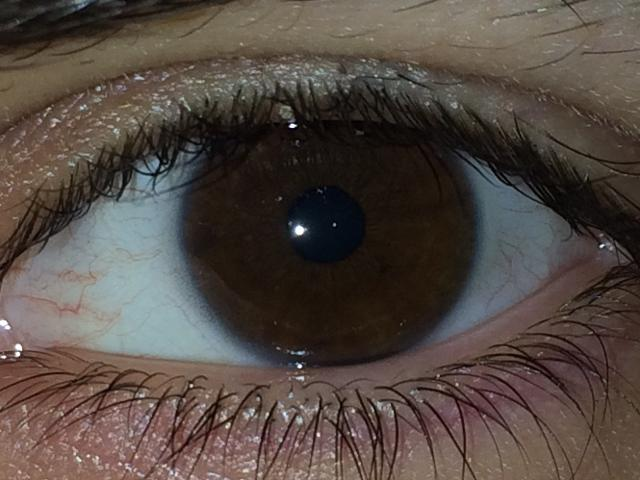
\includegraphics[width=.5\linewidth]{img/iris_vl_escura}
%   \caption{Pigmentação escura.}\label{fig:iris_vl_escura}
% \end{subfigure}%
% \begin{subfigure}{.5\textwidth}
%   \centering
%   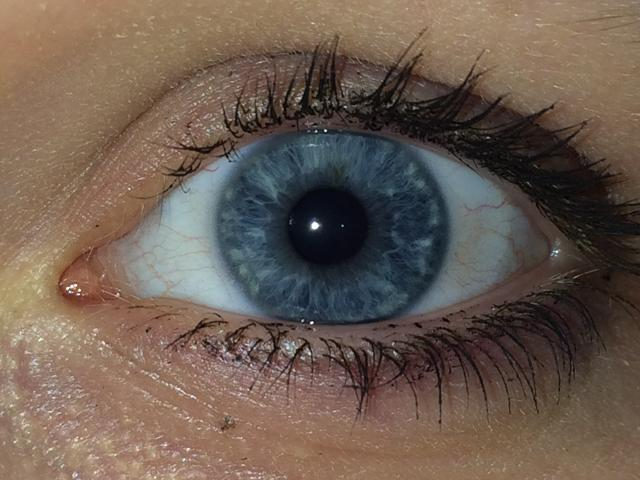
\includegraphics[width=.5\linewidth]{img/iris_vl_clara}
%   \caption{Pigmentação clara.}\label{fig:iris_vl_clara}
% \end{subfigure}
% \caption{Imagens de íris \textit{\acrshort{VL}}.}
% \label{fig:pigmentacoes}
% \end{figure}

% \begin{figure}[h!]
%   \centering
%   \begin{minipage}[b]{0.4\textwidth}
%     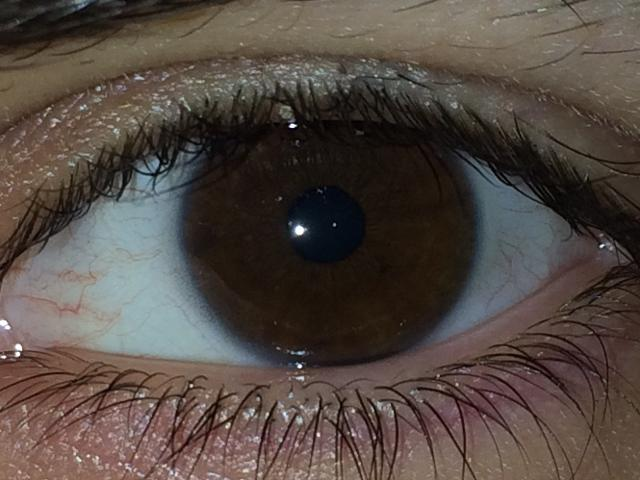
\includegraphics[width=\textwidth]{img/iris_vl_escura.jpg}
%     \caption{Imagem de íris \textit{\arcshort{VL}} com pigmentação escura.} \label{fig:iris_vl_escura}
%   \end{minipage}
%   \hfill
%   \begin{minipage}[b]{0.4\textwidth}
%     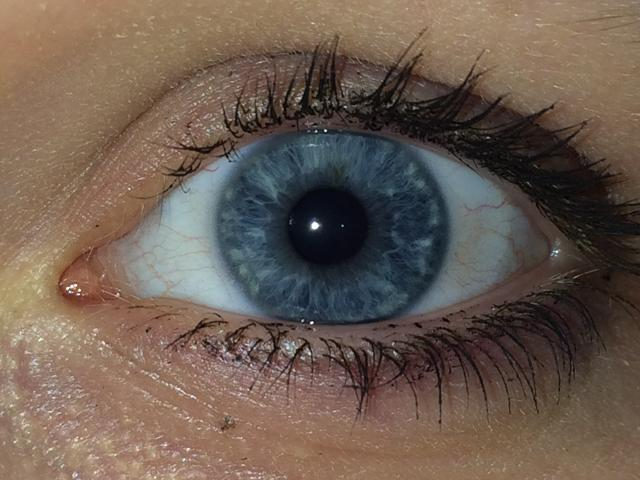
\includegraphics[width=\textwidth]{img/iris_vl_clara.jpg}
%     \caption{Imagem de íris \textit{\arcshort{VL}} com pigmentação clara.}\label{fig:iris_vl_clara}
%   \end{minipage}
% \end{figure}


%%%%%%%%%%%%%%%%%%%%%%%%%%%%%%%%%%%%%%%%%%%%%%%%%%%%%%%%%%%%%%%%%%%%%%%%%%%%%%%%
%%%%%%%%%%%%%%%%%%%%%%%%%%%%%%%%%%%%%%%%%%%%%%%%%%%%%%%%%%%%%%%%%%%%%%%%%%%%%%%%
%%%%%%%%%%%%%%%%%%%%%%%%%%%%%%%%%%%%%%%%%%%%%%%%%%%%%%%%%%%%%%%%%%%%%%%%%%%%%%%%
\section{Processamento de Imagens no Domínio Espacial}

\par Imagem digital é a representação do plano \textit{3D} em \textit{2D}, e corresponde à uma matriz de elementos, chamados \textit{pixels} \cite{gonsalez2006}. \textit{Pixels} são os menores elementos de uma imagem digital, e seus valores recebem o nome de \textit{intensidade de pixel} \cite{gonsalez2006}. Como uma imagem pertence ao plano \textit{2D}, o termo domínio espacial refere-se à própria imagem. A \refEq{eq:espacial:imagem} é a representação matemática de uma imagem, aonde \textit{x} e \textit{y} são inteiros e correspondem à posição dos \textit{pixels} na matriz \cite{gonsalez2006}.

\equacao{eq:espacial:imagem}{I_{x,y} = 
 \begin{bmatrix}
  a_{1,1} & a_{1,2} & \cdots & a_{1,y} \\
  a_{2,1} & a_{2,2} & \cdots & a_{2,y} \\
  \vdots  & \vdots  & \ddots & \vdots  \\
  a_{x,1} & a_{x,2} & \cdots & a_{x,y} 
 \end{bmatrix}}

\par Processar imagens no domínio espacial consiste em aplicar métodos ou operações (T) que modifiquem os valores dos \textit{pixels} diretamente, conforme a \refEq{eq:espacial:proc_esp} \cite{gonsalez2006}.

\equacao{eq:espacial:proc_esp}{I_{saida}(x, y) = T[I_{entrada}(x, y)]}

\par As Subseções \ref{sec:dom_esp:lbp} até \ref{sec:dom_esp:otsu} explicam técnicas de processamento de imagens no domínio espacial.

\subsection{\textit{\acrfull{LBP}}}\label{sec:dom_esp:lbp}

\par \textit{\acrshort{LBP}} é um método que propõpe descritores binários invariantes à rotação para a textura de imagens monocromáticas \cite{ojala2002LBP}. O método consiste em percorrer os \textit{pixels} da imagem de entrada, calcular propriedades da textura local de cada vizinhança do \textit{pixel} referência com raio $R > 0$ e gerar um histograma que mapeia a textura de toda a imagem.

\par As \refEqs{eq:lbp:normal}{eq:lbp:histograma} demonstram como o \textit{\acrshort{LBP}} e o histograma de textura são calculados, respectivamente \cite{ojala2002LBP}\cite{guo2010-CLBP}.

\equacao{eq:lbp:normal}{LBP_{P, R} = \sum_{p=0}^{P-1} s(g_{p} - g_{c})2^P, 
     s(x) = 
     \begin{cases}
         1  & s \geq 0\\
         0  & s < 0  
       \end{cases}
}
       
\par A fórmula é aplicada para cada \textit{pixel} da imagem de entrada. Aonde $g_{c}$ é o valor do \textit{pixel} central da vizinhança sendo calculada, $g_{p}$ o valor do \textit{pixel} dos vizinhos, \textit{P} o total de vizinhos e R o raio da vizinhança. As coordenadas de $g_{p}$ são calculadas pela fórmula ($Rcos(2 \pi p/P)$, $Rsen(2 \pi p/P)$). 

\equacao{eq:lbp:histograma}{H(k) = \sum_{i=1}^{I}\sum_{j=1}^{J}f(LBP_{P,R}(i,j),k), k \in [0, K], \\
    f(x,y) = \begin{cases}
     1 & x = y \\ 
     0 & \text{ caso contrário }
    \end{cases}
}

\par Aonde I e J são a quantidade de linhas e colunas da imagem de entrada, respectivamente, e K o valor máximo do \textit{\acrshort{LBP}}.

\par \textit{\acrshort{LBP}} é bastante utilizado em técnicas de classificação e aplicações em que a textura da imagem é um atributo essencial, como por exemplo \cite{ojala2002LBP}:

\begin{itemize}
    \item Sensoreamento remoto;
    \item Análise de imagens médicas;
    \item Inspeção industrial de superfície;
    \item Qualidade de imagens.
\end{itemize}


\subsection{Filtro \textit{Variância Local}}\label{sec:dom_esp:filtro_std}

\par O filtro \textit{Desvio Padrão Local} consiste em um filtro de domínio espacial que calcula o desvio padrão local de cada \textit{pixel} da imagem de entrada \cite{stdfilt}. O filtro \textit{Variância Local} é, portanto, uma variação do filtro de \textit{Desvio Padrão Local}, que calcula a variância ao invés do desvio padrão.

\par O filtro de \textit{Variância Local} consiste em calcular a variância da vizinhança, dado um elemento estruturante, ao redor do \textit{pixel} de entrada e atribuí-la ao \textit{pixel} de saída, conforme a \refEq{eq:stdfilt}. Essa operação é feita em todos os \textit{pixels} da imagem de entrada.

\equacao{eq:stdfilt}{I_{saida}(x,y) = \frac{1}{N}\sum_{i=1}^{N}(v_{i}^{I_{entrada}(x,y)} - \mu)^2}

\par Aonde N é o número total de vizinhos sendo considerados, $v_{i}^{I_{entrada}(x,y)}$ são os valores de cada vizinho e $\mu$ a média da vizinhança. $I_{saida}(x,y)$ e $I_{entrada}(x,y)$ são o valor do \textit{pixel} em determinada posição, x e y, das imagens de entrada e saída, respectivamente.

\par O filtro \textit{Desvio Padrão Local} é útil para encontrar bordas de objetos em imagens. A \refFig{fig:stdfilt:entrada} ilustra uma imagem de entrada e a \refFig{fig:filtros} os resultados da filtragem dessa imagem pelos filtros de desvio padrão e variância, respectivamente.

\figura[!h]{img/stdfilt_entrada}{Imagem de entrada}{fig:stdfilt:entrada}{width=0.2\textwidth}

\figurasDuplas{h!}{img/stdfilt_std}{img/stdfilt_var}{Resultados da filtragem da \refFig{fig:stdfilt:entrada}}{Com filtro \textit{Desvio Padrão Local}}{Com filtro \textit{Variância Local}}{fig:filtros}{fig:stdfilt:std}{{fig:stdfilt:var}{.5\textwidth}{width=.5\textwidth}}

% \begin{figure}[!h]
%   \centering
%   \begin{minipage}[b]{0.4\textwidth}
%     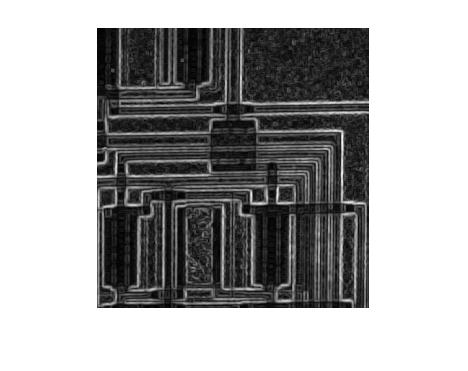
\includegraphics[width=\textwidth]{img/stdfilt_std}
%     \caption{Resultado da filtragem pelo filtro \textit{Desvio Padrão Local}}\label{fig:stdfilt:std}
%   \end{minipage}
%   \hfill
%   \begin{minipage}[b]{0.4\textwidth}
%     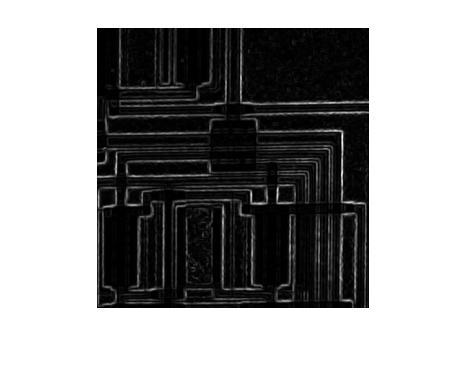
\includegraphics[width=\textwidth]{img/stdfilt_var}
%     \caption{Resultado da filtragem pelo filtro \textit{Variância Local}}\label{fig:stdfilt:var}
%   \end{minipage}
% \end{figure}


\subsection{Método \textit{Otsu}}\label{sec:dom_esp:otsu}

\par Método \textit{Otsu} é um algoritmo de segmentação que separa duas classes em um histograma \cite{otsumethod}. O algoritmo parte do princípio que o histograma de entrada possui duas classes e, então, calcula um limiar que melhor as separa.

\par O cálculo é feito de forma que a variância dentro da mesma classe é mínima e, consequentemente, a variância entre as classes é máxima. As \refEqs{eq:otsu:1}{eq:otsu:5} demonstram matemáticamente os cálculos feitos em cada etapa do algoritmo. Nas equações, ${0, 1, 2, ..., L - 1}$ são todos os \textit{L} possíveis valores do histograma, $p_{i}$ as probabilidades em que esses valores aparecem e \textit{t} o limiar sendo considerado para os cálculos. O limiar \textit{T} vai ser algum valor no intervalo $0 < T < L - 1$. As etapas do algoritmo são descritas abaixo:

\begin{enumerate}
    \item Calcular o histograma e as probablidades de cada valor do histograma;
    \item 
        Para cada $t = 0 \text{ até } L-1$:
        \begin{enumerate}
            \item Atualizar as probabilidades e as médias de cada classe;
            \item Calcular a variância entre as classes;
        \end{enumerate}
    \item Escolher o limiar \textit{T} de forma que seja a maior variância calculada.
\end{enumerate}

\equacao{eq:otsu:1}{\omega_{1}(t) = \sum_{i=0}^{t-1}p(i)}

\equacao{eq:otsu:2}{\omega_{2}(t) = \sum_{i=t}^{L-1}p(i)}

\equacao{eq:otsu:3}{\sigma_{b}^{2}(t) = \omega_{1}(t)\omega_{2}(t)(\mu_{1} - \mu_{2})^2}

\equacao{eq:otsu:4}{\mu_{1}(t) = \frac{1}{\omega_{1}(t)}\sum_{i=0}^{t-1}ip(i)}

\equacao{eq:otsu:5}{\mu_{2}(t) = \frac{1}{\omega_{2}(t)}\sum_{i=t}^{L-1}ip(i)}

\par Aonde $\omega_{1}(t)$ e $\omega_{2}(t)$ são as probabilidades de cada classe; $\sigma_{b}^{2}(t)$ a variância entre as duas classes; e $\mu_{1}(t)$ e $\mu_{2}(t)$ as médias das classes.

\par Sua principal aplicação é em processamento de imagens, e consiste em binarizar imagens em escala de cinza. A binarização é feita calculando o histograma da imagem e então encontrando o limiar (intensidade de \textit{pixel}) que melhor separa o fundo e o primeiro plano das imagens \cite{gonsalez2006}. A \refFig{fig:otsu} ilustra imagens antes e depois da binarização utilizando o método \textit{Otsu}.

\figurasDuplas{h!}{img/stdfilt_entrada}{img/otsu_binaria}{Processo de binarização de imagens utilizando o método \textit{Otsu}}{Imagem original}{Imagem binarizada}{fig:otsu}{fig:otsu:org}{{fig:otsu:bin}{.5\textwidth}{width=.5\textwidth}}

% \begin{figure}[h!]
% \centering
% \begin{subfigure}{.5\textwidth}
%   \centering
%   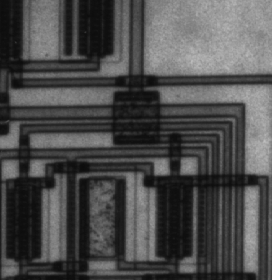
\includegraphics[width=.5\linewidth]{img/stdfilt_entrada.png}
%   \caption{Imagem antes da binarização.}
% \end{subfigure}%
% \begin{subfigure}{.5\textwidth}
%   \centering
%   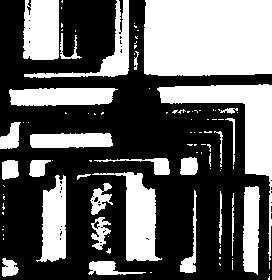
\includegraphics[width=.5\linewidth]{img/otsu_binaria.png}
%   \caption{Imagem binarizada.}
% \end{subfigure}
% \caption{Processo de binarização de imagens.}
% \label{fig:otsu}
% \end{figure}

\section{Processamento Morfológico de Imagens}\label{sec:morf}

\par Morfologia matemática é o estudo de estruturas geométricas. Operações morfológicas aplicadas em imagens consistem no processamento de regiões baseados em suas formas \cite{gonsalez2006}. 

\par A operação consiste em aplicar um elemento estruturante em uma imagem de entrada de forma a gerar uma imagem de saída. Os elementos estruturantes são matrizes e podem ter inúmeros formatos e tamanhos, sendo círculos e quadrados os mais utilizados.

\par O elemento estruturante é sobreposto em todos os \textit{pixels} da imagem, de forma que todos os elementos com valor 1 no elemento são considerados na região sobreposta da imagem. Para todo elemento estrututante, é atribuído um \textit{ponto âncora}, que é o \textit{pixel} da região sobreposta da imagem de entrada processado. A \refFig{fig:kernel_morfo} ilustra um elemento estruturante.

\figura[!h]{img/kernel}{Exemplo de elemento estruturante. O elemento central destacado é o \textit{ponto âncora}}{fig:kernel_morfo}{width=0.2\textwidth}

\par Operações morfológicas são aplicadas em imagens para inúmeras aplicações, mas as principais são \cite{erosionDilationOpencv}:

\begin{itemize}
    \item Isolar elementos individuais;
    \item Juntar elementos que podem ser do mesmo objeto;
    \item Remover ruídos;
    \item Achar buracos ou sobreposições.
\end{itemize}

\par As duas principais operações morfológicas são a dilatação e erosão, e são explicadas nas Seções \ref{sec:morf:dil} e \ref{sec:morf:ero}, respectivamente.

\subsection{Dilatação} \label{sec:morf:dil}

\par Operação morfológica que aumenta regiões mais claras, ou diminui regiões mais escuras, da imagem de entrada \cite{gonsalez2006}. Pode ser utilizada também para calcular máximos locais de imagens.

\par O elemento estrututante é sobreposto em cada um dos \textit{pixels} da imagem de entrada, o máximo local da região sobreposta é calculado, e por fim, esse máximo é atribuído à imagem de saída na \textit{posição âncora} do elemento estruturante. A \refFig{fig:processo_dilatacao} ilustra as etapas descritas acima, considerando o elemento estrututante da \refFig{fig:kernel_morfo}.

\figura[!h]{img/dilatacao}{Resultado da etapa de dilatação. O fundo amarelo corresponde ao elemento estrututante e o verde ao \textit{ponto âncora} substituído pelo máximo valor da região sobreposta}{fig:processo_dilatacao}{width=0.4\textwidth}

\par A \refFig{fig:dil} ilustra uma imagem de entrada para a operação de dilatação e a imagem de saída resultante, respectivamente.

\figuraBib[h!]{img/dil}{Imagem de entrada e saída da operação de dilatação}{erosionDilationOpencv}{fig:dil}{width=0.4\textwidth}%

\subsection{Erosão} \label{sec:morf:ero}

\par Operação morfológica que diminui regiões mais claras, ou aumenta regiões mais escuras, da imagem de entrada \cite{gonsalez2006}. Pode ser utilizada também para calcular mínimos locais de imagens.

\par Possui procedimentos parecidos com a operação de dilatação, mas ao invés de calcular os máximos das regiões sobrepostas pelo elemento estrututante, calcula os mínimos.

\par A \refFig{fig:ero} ilustra uma imagem de entrada para a operação de erosão e a imagem de saída resultante, respectivamente.

\figuraBib[!h]{img/ero}{Imagem de entrada e saída da operação de erosão}{erosionDilationOpencv}{fig:ero}{width=0.4\textwidth}%

%%%%%%%%%%%%%%%%%%%%%%%%%%%%%%%%%%%%%%%%%%%%%%%%%%%%%%%%%%%%%%%%%%%%%%%%%%%%%%%%
%%%%%%%%%%%%%%%%%%%%%%%%%%%%%%%%%%%%%%%%%%%%%%%%%%%%%%%%%%%%%%%%%%%%%%%%%%%%%%%%
%%%%%%%%%%%%%%%%%%%%%%%%%%%%%%%%%%%%%%%%%%%%%%%%%%%%%%%%%%%%%%%%%%%%%%%%%%%%%%%%
\section{Filtragem de Imagens} \label{sec:fundamentacao:filtragem}

\par Filtros são processos que modificam sinais de entrada. Como imagens são sinais, o processo de filtrar imagens consiste em modificá-las \cite{gonsalez2006}. Filtros podem ser usados para remover componentes indesejados, realçar componentes desejados ou até para extrair informações ou atributos do sinais sendo processados \cite{loggabor-kovesi}.

\par Imagens podem ser filtradas tanto no domínio do espaço quanto da frequência. A filtragem no domínio espacial consiste em realizar o processo de convolução \textit{2D} por meio de filtros espaciais, chamados de máscaras ou \textit{kernel}\cite{oppenheim2013signals}. A convolução \textit{2D} pode ser representada matemáticamente pela \refEq{eq:filtragem:convolucao}, aonde $g$ é a convolução, $H$ o \textit{kernel} e $I$ a imagem sendo filtrada\cite{gonsalez2006}. A \refEq{eq:filtragem:convolucao_simplificada} é a versão simplificada da \refEq{eq:filtragem:convolucao}. 

\equacao{eq:filtragem:convolucao}{g(x,y) = \sum_{s=-a}^{a}\Bigg(\sum_{t=-b}^{b}H(s,t)I(x-s,y-t)\Bigg)}

\equacao{eq:filtragem:convolucao_simplificada}{g = I*H}

\par Já a filtragem no domínio da frequência, consiste apenas na multiplicação da imagem e do \textit{kernel} transformados para o domínio da frequência pela \textit{Transformada de Fourier} (\textit{F(.)}) \cite{gonsalez2006}. A \refEq{eq:filtragem:relacao} ilustra a relação entre as filtragens nos dois espaços.

\equacao{eq:filtragem:relacao}{I*H \iff F(I) \cdot F(H)}

\par Filtragem no domínio da frequência é útil quando deseja-se remover ou realçar um intervalo de frequências da imagem.

\subsection{\textit{Filtro Log-Gabor}}\label{sec:fundamentacao:filtragem:loggabor}

\par O filtro \textit{Log-Gabor} é uma adaptação do filtro \textit{Gabor}, mas na escala logarítmica, e é um filtro linear passa banda \cite{field1987-loggabor}. Possui duas características que o diferem: não possue componentes \textit{DC} e não pode ser representado por uma máscara no domínio do espaço, de forma que é exclusivo ao domínio da frequência \cite{loggabor-kovesi}. Assim como o filtro \textit{Gabor}, é muito utilizado para a extração de atributos e codificação de íris \cite{masek2003}.

\par A função de ativação do filtro \textit{Log-Gabor} é representada pela \refEq{eq:filtragem:loggabor}. Aonde $\sigma$ controla a largura de banda e $\omega_{0}$ a frequência central do filtro. Já a \refFig{fig:loggabor}, ilustra a função de ativação do filtro na escala linear.

\equacao{eq:filtragem:loggabor}{H(\omega) = e^{\frac{-log(\omega/\omega_{0})^{2}}{2log(\sigma)^{2}}}}

\figura[!h]{img/loggabor}{Função de ativação do filtro \textit{Log-Gabor} na escala linear}{fig:loggabor}{width=0.5\textwidth}


%%%%%%%%%%%%%%%%%%%%%%%%%%%%%%%%%%%%%%%%%%%%%%%%%%%%%%%%%%%%%%%%%%%%%%%%%%%%%%%%
%%%%%%%%%%%%%%%%%%%%%%%%%%%%%%%%%%%%%%%%%%%%%%%%%%%%%%%%%%%%%%%%%%%%%%%%%%%%%%%%
%%%%%%%%%%%%%%%%%%%%%%%%%%%%%%%%%%%%%%%%%%%%%%%%%%%%%%%%%%%%%%%%%%%%%%%%%%%%%%%%